\documentclass[12pt,a4paper]{article}
\usepackage[utf8]{inputenc}
\usepackage[margin=1in]{geometry}
\usepackage{graphicx}
\usepackage{float}
\usepackage{amsmath}
\usepackage{listings}
\usepackage{xcolor}

% Code listing style
\lstset{
    language=C++,
    basicstyle=\ttfamily\footnotesize,
    keywordstyle=\color{blue},
    commentstyle=\color{green},
    stringstyle=\color{red},
    numbers=left,
    numberstyle=\tiny,
    frame=single,
    breaklines=true
}

\begin{document}

% Front Page
\begin{titlepage}
  \centering
  \vspace*{3cm}

  {\Huge\bfseries CSE 406 – Lab Report 1: First Come First Serve (FCFS) Scheduling Algorithm \par}
  \vspace{2.5cm}

  \noindent
  \begin{minipage}[t]{0.48\textwidth}
    {\large\bfseries Submitted By:}\\[0.5em]
    \Large
    Sharif Md. Yousuf \\
    ID: 22101128 \\
    Section: C-2 \\
    4th Year, 1st Semester \\
    Spring 2025
  \end{minipage}
  \hfill
  \begin{minipage}[t]{0.48\textwidth}
    {\large\bfseries Submitted To:}\\[0.5em]
    \Large
    Atia Rahman Orthi \\
    Lecturer \\
    Department of Computer Science \& Engineering \\
    University of Asia Pacific
  \end{minipage}

  \vfill

  {\Large\bfseries Date of Submission:} \\[0.5em]
  {\LARGE\bfseries 23 July, 2025 (Wednesday)}

  \vspace*{2cm}
\end{titlepage}

\section{Problem Statement}
A program is needed to efficiently implement the First Come First Serve (FCFS) CPU scheduling algorithm. The algorithm should schedule processes according to their arrival times, meaning that the first process to arrive gets executed first. The implementation must first handle cases of processes arriving at different times and then compute the major scheduling parameters of completion time, turnaround time, and waiting time for each process.

\section{Objective}
In this lab we:
\begin{itemize}
    \item Understood the working mechanism of the FCFS scheduling algorithm
    \item Implemented an optimized version that sorts processes by arrival time for better efficiency
    \item Calculated and displayed scheduling metrics for performance analysis
    \item Analyzed the advantages and limitations of non-preemptive FCFS scheduling
\end{itemize}

\section{Source Code Screenshot}
\begin{figure}[H]
    \centering
    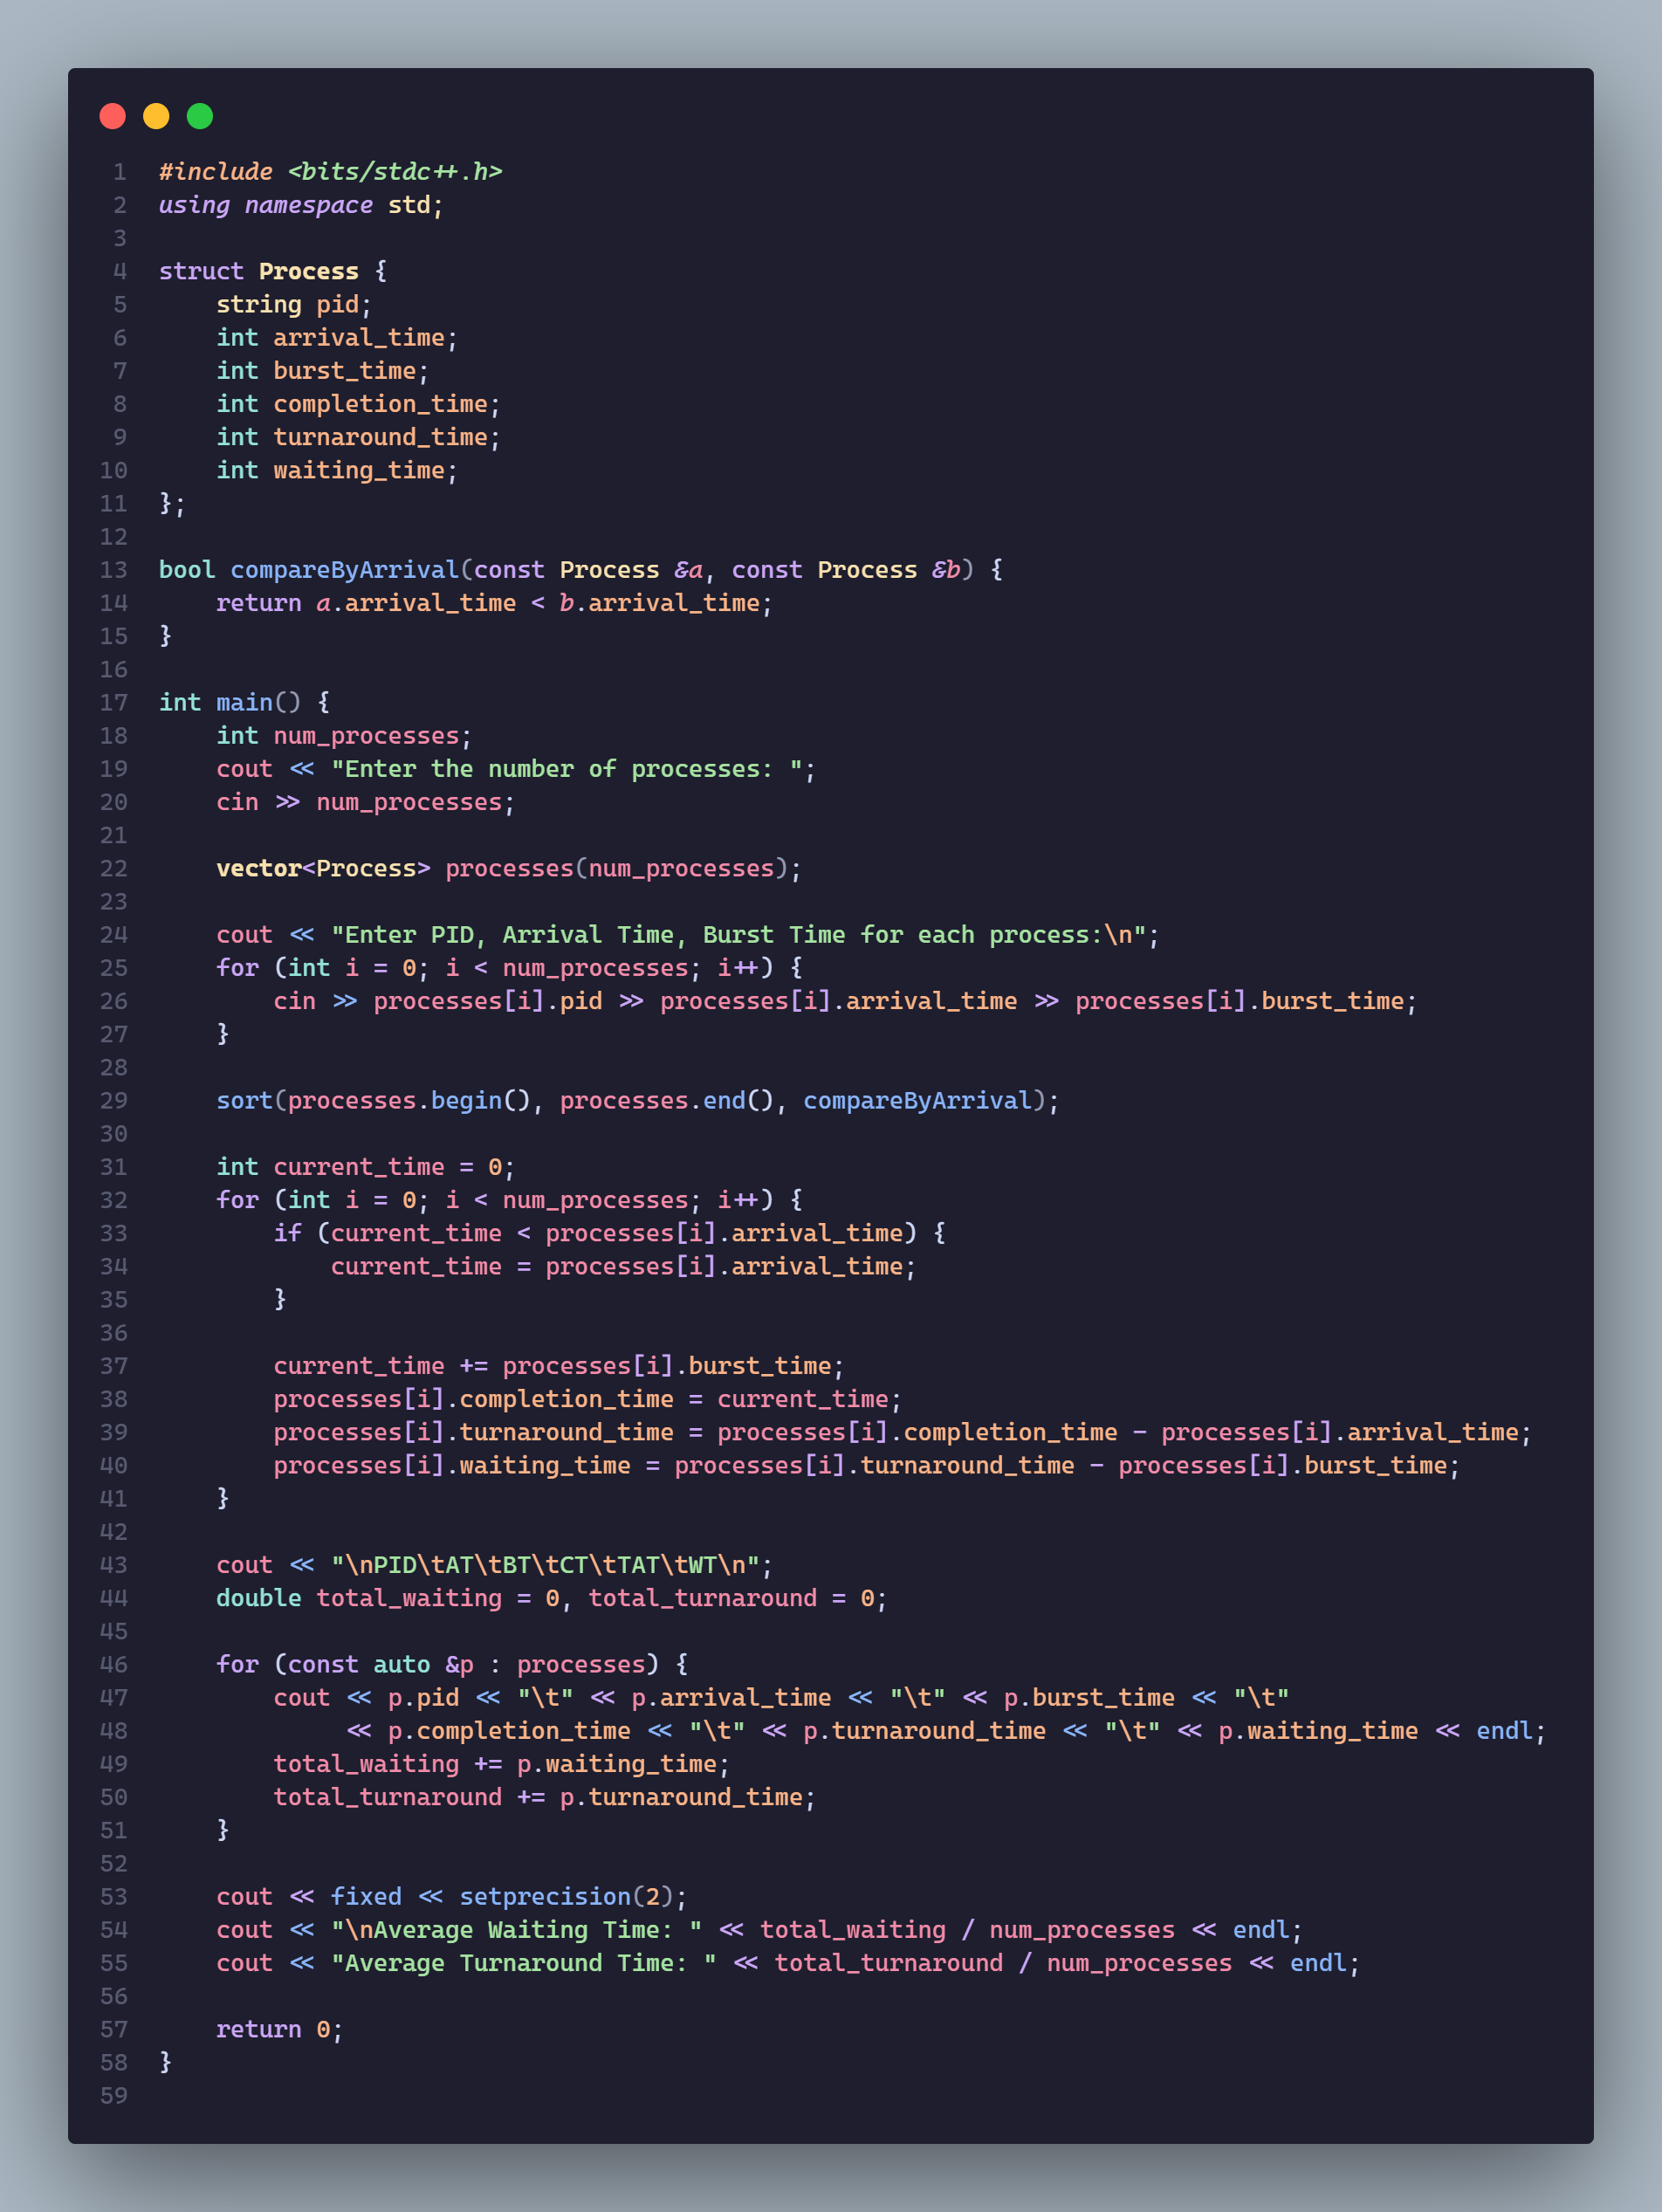
\includegraphics[width=0.8\textwidth]{code.png}
    \caption{FCFS Optimized Algorithm Source Code}
    \label{fig:fcfs_source}
\end{figure}

\section{Output Screenshot}
\begin{figure}[H]
    \centering
    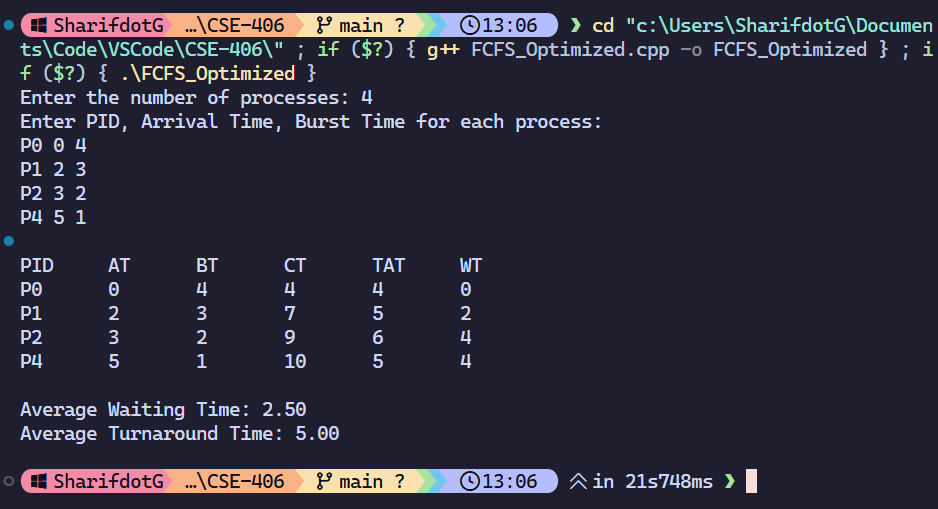
\includegraphics[width=0.8\textwidth]{Screenshot 2025-07-23 130728.png}
    \caption{FCFS Algorithm Execution Output}
    \label{fig:fcfs_output}
\end{figure}

\section{Discussion}
The implemented FCFS optimized algorithm demonstrates several key improvements over a basic implementation. By sorting processes according to their arrival times at the beginning, the algorithm ensures proper execution order without repeatedly searching for the next process to execute.

The algorithm works by first collecting all process information, then sorting them by arrival time using a custom comparator function. During execution, it maintains a current time counter and processes each job in order. If the CPU is idle (current time is less than the next process arrival time), it advances the time to the next process arrival.

Key observations from the implementation include:
\begin{itemize}
    \item Time complexity is reduced to O(n log n) due to sorting, compared to O(n²) in naive implementations
    \item The algorithm handles CPU idle time effectively by jumping to the next arrival time
    \item Waiting time calculation is straightforward: turnaround time minus burst time
    \item The non-preemptive nature means once a process starts, it runs to completion
\end{itemize}

The results show that FCFS provides predictable scheduling behavior but may not be optimal for minimizing average waiting time, especially when long processes arrive before shorter ones.

\section{Conclusion}
The FCFS optimized scheduling algorithm successfully demonstrates the fundamental principles of CPU scheduling. While simple to understand and implement, the algorithm has inherent limitations such as the convoy effect, where short processes wait behind long ones. However, its fairness and simplicity make it suitable for systems where predictable execution order is more important than optimal performance metrics. The optimization through sorting provides better algorithmic efficiency while maintaining the core FCFS behavior.

\end{document}